% Use only LaTeX2e, calling the article.cls class and 12-point type.

\documentclass[11pt]{article}

% Users of the {thebibliography} environment or BibTeX should use the
% scicite.sty package, downloadable from *Science* at
% www.sciencemag.org/about/authors/prep/TeX_help/ .
% This package should properly format in-text
% reference calls and reference-list numbers.

%\usepackage{scicite}

% Use times if you have the font installed; otherwise, comment out the
% following line.

%\usepackage{times}
\usepackage{cite}
%\usepackage{epsfig}
\usepackage[tight,footnotesize]{subfigure}
\usepackage{calc}
\usepackage{amstext}
\usepackage[cmex10]{amsmath}
%\usepackage{amsthm}
\usepackage{multicol}
\usepackage{pslatex}
\usepackage{color}
\usepackage{graphicx}
\usepackage[small]{caption}
\usepackage{booktabs}
\usepackage{epstopdf}
\usepackage{float}
\usepackage[margin=1.0in]{geometry}
%\usepackage{flushend}

% The preamble here sets up a lot of new/revised commands and
% environments.  It's annoying, but please do *not* try to strip these
% out into a separate .sty file (which could lead to the loss of some
% information when we convert the file to other formats).  Instead, keep
% them in the preamble of your main LaTeX source file.


% The following parameters seem to provide a reasonable page setup.

%\topmargin -1.5cm
%\oddsidemargin 0.2cm
%\textwidth 16cm 
%\textheight 22cm
%\footskip 0.0cm


%The next command sets up an environment for the abstract to your paper.

\newenvironment{sciabstract}{%
\begin{quote} \bf}
{\end{quote}}


% If your reference list includes text notes as well as references,
% include the following line; otherwise, comment it out.

\renewcommand\refname{References}

% The following lines set up an environment for the last note in the
% reference list, which commonly includes acknowledgments of funding,
% help, etc.  It's intended for users of BibTeX or the {thebibliography}
% environment.  Users who are hand-coding their references at the end
% using a list environment such as {enumerate} can simply add another
% item at the end, and it will be numbered automatically.

\newcounter{lastnote}
\newenvironment{scilastnote}{%
\setcounter{lastnote}{\value{enumiv}}%
\addtocounter{lastnote}{+1}%
\begin{list}%
{\arabic{lastnote}.}
{\setlength{\leftmargin}{.22in}}
{\setlength{\labelsep}{.5em}}}
{\end{list}}


% Include your paper's title here
%\vskip -2in
\title{Energy-optimal replication for periodic real-time tasks}


% Place the author information here.  Please hand-code the contact
% information and notecalls; do *not* use \footnote commands.  Let the
% author contact information appear immediately below the author names
% as shown.  We would also prefer that you don't change the type-size
% settings shown here.

\author
{Xiaolong Cui\\
\normalsize{mclarencui@cs.pitt.edu}\\
%\\
%\normalsize{$^\ast$To whom correspondence should be addressed; E-mail:  jsmith@wherever.edu.}
}

% Include the date command, but leave its argument blank.

\date{}



%%%%%%%%%%%%%%%%% END OF PREAMBLE %%%%%%%%%%%%%%%%



\begin{document} 

% Double-space the manuscript.

%\baselineskip24pt

% Make the title.

\maketitle 



% Place your abstract within the special {sciabstract} environment.

%\begin{sciabstract}
%  This document presents a number of hints about how to set up your
%  {\it Science\/} paper in \LaTeX\ .  We provide a template file,
%  \texttt{scifile.tex}, that you can use to set up the \LaTeX\ source
%  for your article.  An example of the style is the special
%  \texttt{\{sciabstract\}} environment used to set up the abstract you
%  see here.
%\end{sciabstract}



% In setting up this template for *Science* papers, we've used both
% the \section* command and the \paragraph* command for topical
% divisions.  Which you use will of course depend on the type of paper
% you're writing.  Review Articles tend to have displayed headings, for
% which \section* is more appropriate; Research Articles, when they have
% formal topical divisions at all, tend to signal them with bold text
% that runs into the paragraph, for which \paragraph* is the right
% choice.  Either way, use the asterisk (*) modifier, as shown, to
% suppress numbering.

\section{Introduction}
\label{sec:intro}
As our reliance on IT continues to increase, the complexity and urgency of the problems our society will face 
in the future drives us to build more powerful and accessible computer systems. Among the different types of 
computer systems, High Performance Computing (HPC) and Cloud Computing systems are the two most powerful ones. 
For both, the computing power attributes to the massive amount of parallelism, which is enabled by 
the massive amount of CPU cores, memory modules, communication devices, storage components, etc. 

Since CPU frequency flattened out in early 2000s, parallelism has become the ``golden rule" to boost performance. 
In HPC, Terascale performance was achieved in the late 90’s with fewer than 10,000 heavyweight single-core processors. 
A decade later, petascale performance required about ten times more processors with multiple cores on each processor. Nowadays, a race
is underway to build the world's first exascale machine to accelerate scientific discoveries and breakthroughs. It is 
projected that an exascale machine will achieve billion-way parallelism by using one million sockets each supporting 
1,000 cores~\cite{doe_ascr_exascale_2011,top_ten_2014}. 

Similar trend is happening in Cloud Computing. 
As the demand for Cloud Computing accelerates, cloud service providers  
will be faced with the need to expand their underlying infrastructure to ensure the expected levels of performance, reliability and cost-effectiveness. 
As a result, lots of large-scale data centers have been and are being built by IT companies
to exploit the power and economies of scale. 
For example, Google, Facebook, and Rackspace have hundreds of thousands 
of web servers in dedicated data centers to support their business. 

Unfortunately, several challenging issues come with the increase in system scale. As today's HPC and Cloud Computing systems grow to 
meet tomorrow's compute power demand, the behavior of the systems will be increasingly difficult to specify, predict and manage. 
This upward trend, in terms of scale and complexity, has a direct negative effect on the overall system reliability. 
%Even with the expected improvement in the reliability of future computing technology, the rate of system level failures will 
%dramatically increase with the number of components, possibly by several orders of magnitude. 
At the same time, the rapid 
growing power consumption, as a result of the increase in system components, is another major concern. 
%It is reported that 
%the power required to run the machines as well as cool them has become the largest cost factor in a large-scale system's operating 
%expenses.  
At future extreme-scale, failure would become a norm rather than an exception, 
driving the system to significantly lower efficiency with unprecedented amount of power consumption. 

\section{Problem Statement}

The system scale needed to address our future computing needs will come at the cost of increasing complexity, unpredictability, 
and operating expenses. As we approach future extreme-scale computing, two of the biggest challenges will be system resilience and power 
consumption, both being direct consequences of the dramatic increase in the number of system components~\cite{exa_challenge_2010,snir2014addressing}. 

Regardless of the reliability of individual component, the system level failure rate will continue to increase as the number of 
components increases, possibly by several orders of magnitude. It is projected that the Mean Time Between Failures (MTBF) of future extreme-scale systems will be at the order of hours or even minutes, meaning 
that many failures will occur every day~\cite{Bergman08exascalecomputing}. Without an efficient fault tolerance mechanism, faults will be so frequent that the applications running on the 
systems will be continuously interrupted, requiring the execution to be restarted every time there is a failure. 

Also thanks to the continuous growth in system components, there has been a steady rise in power consumption in large-scale distributed systems. 
In 2005, the peak power consumption of a single supercomputer reached 3.2 Megawatts. This number was doubled only after 5 years, and reached 17.8 
Megawatts with a machine of 3,120,000 cores in 2013. Recognizing this rapid upward trend, the U.S. Department of Energy has set 20 
megawatts as the power limit for future exascale systems, 
challenging the research community to provide a 1000x improvement in performance with only a 10x increase in power~\cite{exa_challenge_2010}. 
This huge imbalance makes system power a leading design constraint on the path to exascale. 

Today, two approaches exist for fault tolerance. The first approach is rollback recovery, which rolls back and restarts the execution 
every time there is a failure. This approach is often equipped with checkpointing to periodically save the execution state to a 
stable storage so that execution can be restarted from a recent checkpoint in the case of a failure~\cite{Elnozahy:02:Survey,kalaiselvi_sadhana_2000,Chandy:1985:DSD:214451.214456}. 
Although checkpointing is the most widely used technique in today's HPC systems, it may not scale to 
future extreme-scale systems~\cite{ferreira_sc_2011,elnozahy_dsc_2004,4367962}. Given the anticipated increase in system level failure rates and the time to checkpoint large-scale 
compute-intensive and data-intensive applications, the time required to periodically checkpoint an application 
and restart its execution will approach the system's MTBF~\cite{Cappello:2009:TER:1640402.1640428}. Consequently, applications will make little forward progress, thereby 
reducing considerably the overall system efficiency. 

The second approach, referred to as process replication, exploits hardware redundancy and executes multiple instances of the same task 
in parallel to overcome failure and guarantee that at least one task instance reaches completion~\cite{bartlett_1981_nonstop,tsai_isads_2011,ferreira_sc_2011}. Although this approach is extensively used 
to deal with failures in 
Cloud Computing and mission critical systems, it has 
never been used in any HPC system due to its low system efficiency. To replicate each process, process replication requires 
at least double the amount of compute nodes, which also increases the power consumption proportionally. 

Based on above analysis, neither of the two approaches is efficient for future extreme-scale systems. And unfortunately, neither 
of them addresses the power cap issue. 
Achieving high resilience to failures under strict power constraints is a daunting and critical challenge that requires new 
computational models with scalability, adaptability, and power-awareness in mind. 
 
\section{Research Overview}

There is a delicate interplay between fault tolerance and power consumption. Checkpointing and process replication require 
additional power to achieve fault tolerance. Conversely, it has been shown that lowering supply voltages, a commonly used 
technique to conserve power, increases the probability of transient faults~\cite{chandra2008defect,zhao2008reliability}. The trade-off between fault free operation and 
optimal power consumption has been explored in the literature~\cite{meneses2014energy,mills2014energy}. Limited insights have emerged, however, with respect to how 
adherence to application's desired QoS requirements affects and is affected by the fault tolerance and power consumption 
dichotomy. In addition, abrupt and unpredictable changes in system behavior may lead to unexpected fluctuations in performance, 
which can be detrimental to applications’ QoS requirements. The inherent instability of extreme-scale computing systems, 
in terms of the envisioned high-rate and diversity of faults, together with the demanding power constraints under which 
these systems will be designed to operate, calls for a 
reconsideration of the fault tolerance problem.

To this end, Mills, Znati, and Melhem have proposed a novel computational model, referred to as Shadow Replication, as a  
power-aware approach to achieve high-levels of resilience through forward progress~\cite{mills_2014_icnc,mills_2014_pdp,mills2014power}. Based on Dynamic Voltage and Frequency Scaling (DVFS)~\cite{Orgerie:2014:STI:2597757.2532637,4658633,LeSueur:2010:DVF:1924920.1924921}, Mills studied the computational model and its performance in terms of completion time and energy consumption in HPC systems. Through the use of analytical models, simulations, and experimentation, Mills demonstrated that Shadow Replication can achieve resilience more efficiently than both checkpointing and traditional replication when power is limited. However, in Mills' work Shadow Replication is limited to the use of DVFS, which has been shown to have multiple issues that question its viability~\cite{Eyerman:2011:FDU:1952998.1952999,Keller:EECS-2015-257,chandra2008defect,zhao2008reliability}. In addition, Mills' study is limited to HPC systems and focuses exclusively on minimizing energy consumption with constraints on time to completion. In contrast, QoS requirements for various computing systems can be expressed in multiple dimensions that go beyond time and energy. At the same time, an implementation is needed to verify the computational model both with and without failures. 


%In this thesis, our research objective is to simultaneously address the power and resilience challenges for future extreme-scale 
%systems so that both system efficiency and application QoS are guaranteed.
%To this end, we propose an adaptive and power-aware computational model, referred to as Lazy Shadowing, as an efficient and 
%scalable alternative to achieve high-levels of resilience, through forward progress, in extreme-scale, failure-prone 
%computing environments. 
%The basic tenet of Lazy Shadowing is to associate with each main process a suite of “shadows” whose size depends on the 
%``criticality" of the application and its performance requirements. Each shadow process is an exact replica of the original 
%main process. To tolerate failures, the main process and its associated shadow processes will execute in parallel, but on 
%different compute nodes. 
%The shadows initially execute at a reduced rate %via Dynamic Voltage Frequency and Scaling (DVFS) 
%to save power. 
%If the main process completes the task successfully, we will 
%terminate the shadows immediately. If the main process fails, however, we will promote one of the shadow processes to be a 
%new main process and possibly increase its execution rate to mitigate delay.

To address the above limitations, this thesis builds on the computational model of Shadow Replication, and seeks to simultaneously address the power and resilience challenges for future extreme-scale systems while guaranteeing system efficiency and application QoS.
Specifically, this thesis tries to answer 4 questions: 1) is Shadow Replication general enough to achieve objectives beyond time to completion; %, such as multiple simultaneous requirements defined in a SLA in the Cloud; 
2) how to enable Shadow Replication when DVFS is not viable, and ensure forward progress in failure-prone, extreme-scale systems; 3) is the computational model realistic in real environments; and 4) how to make the computational model reflective of the propensity of the processing elements to failures and adaptive to different environments and requirements.
With these questions in mind, 
I have studied different techniques to embody and augment the model, and developed analytical frameworks for different objectives in the Cloud and HPC environments~\cite{cui_2014_closer,cui_en7085151,cui_2016_scalcom}.
%Previously, we have formally defined the computational model, studied possible techniques to realize and optimize the idea, and 
%built analytical models for performance evaluation. 
To complete my thesis, I propose to extend the study in the following two aspects.
Firstly, I propose to implement a prototype in the context of Message Passing Interface (MPI), to validate the 
computational model as well as measure its performance in real environment. Secondly, I propose to study  
``smart shadowing" which adapts to the system configuration, application characteristics, and QoS requirement.
In summary, my thesis will consist of the following main components.

%\subsection{Lazy Shadowing: a novel fault-tolerant computational model (completed)}

%The basic tenet of Lazy Shadowing is to associate with each main process a suite of “shadows” whose size depends on the 
%``criticality" of the application and its performance requirements. Each shadow process is an exact replica of the original 
%main process. To tolerate failures, the main process and its associated shadow processes will execute in parallel, but on 
%different compute nodes. 
%The shadows initially execute at a reduced rate %via Dynamic Voltage Frequency and Scaling (DVFS) 
%to save power. 
%If the main process completes the task successfully, we will 
%terminate the shadows immediately. If the main process fails, however, we will promote one of the shadow processes to be a 
%new main process and possibly increase its execution rate to mitigate delay. This continues until the task completes. 

%Given that the failure rate of an individual node is much lower than the aggregate system failure, it is very likely that 
%the main process will always complete its execution successfully, thereby achieving fault tolerance at a significantly reduced 
%cost of power. Consequently, the high probability that shadows never have to complete the full task, coupled with the fact that 
%they initially only consume a minimal amount of power, dramatically increases a power-constrained system's tolerance to failure.

\subsection{Reward-based optimal Shadow Replication (completed)}
Shadow Replication is a flexible computational model that can achieve multi-dimensional QoS requirements. 
The major challenge resides in determining jointly the execution rates of all task instances, 
both before and after a failure occurs, with the objective to optimize performance, resilience, power consumption, or their combinations.
In this work we focus on the Service Level Agreement (SLA) requirements in the Cloud and develop a reward-based analytical framework, in order to derive the optimal execution rates for maximizing reward and minimizing energy 
costs under strict completion time constraints~\cite{cui_2014_closer,cui_en7085151}. 

%To define the reward-based analytical framework, we first define a failure model that considers the failure distribution of each process, and a power model that describes the power consumption characteristics under different states. Based on the failure model and power model, we then derive the expected income as a function of completion time, and the expected energy cost as a product of power and time. Lastly, the reward is defined as the optimization objective to balance between completion time and energy cost.  



\subsection{Lazy Shadowing (completed)}

Enabling Shadow Replication for resiliency in extreme-scale computing brings about a number of challenges and design decisions, including the applicability of this concept to a large number of tasks executing in parallel, 
the effective way to control shadows’ execution rates, and the runtime mechanisms and communications support to ensure efficient 
coordination between a main and its shadow. Taking into consideration the main characteristics of compute-intensive and 
highly-scalable applications, 
we devise novel ideas of shadow collocation and shadow leaping, and integrate them with Shadow Replication to form a more efficient and scalable paradigm that we call Lazy Shadowing~\cite{cui_2016_scalcom}.
%we design two novel techniques, referred to as shadow collocation and shadow leaping, 
%in order to achieve high tolerance to failures while minimizing delay and power consumption.

%To control the processes' execution rate, DVFS can be applied while each process resides on one core exclusively. 
%The effectiveness of DVFS, however, may be markedly 
%limited by the granularity of voltage control, the number of frequencies available, and the negative effects on 
%reliability. 
%An alternative is to collocate multiple processes on each core while keeping all the cores executing at maximum frequency. 
%Then time sharing can be used to achieve the desired execution rates for each collocated process. 
%Since this approach collocates multiple processes on a core, it simultaneously reduces the number of compute nodes and 
%the power consumption. 
%
%Furthermore, we identify a unique opportunity that ensures forward progress in failure-prone environments. Since each shadow process is associated with a main process, the lagging shadow can benefit from the faster execution 
%of the main with minimal overhead. Specifically, when a failure occurs, Lazy Shadowing takes advantage of 
%the recovery time and leaps forward each shadow by copying states from its associated main. This technique not only achieves forward 
%progress for the shadow processes at minimized power and delay, but also reduces the recovery time after each failure.

\subsection{lsMPI: an implementation in MPI (in progress)}

Though Lazy Shadowing has been evaluated analytically, a real implementation 
is necessary for validation and performance measurement in real systems. I am implementing a prototype of Lazy 
Shadowing as a runtime for Message Passing Interface (MPI). %, which is the de facto programming paradigm for HPC. 
%Instead of 
%a full-feature MPI implementation, the runtime is designed to be a separate layer between MPI and user application, in order 
%to take advantage of existing MPI performance optimizations that numerous researches have spent years on. 
The runtime will spawn 
the shadow processes at initialization phase, manage the coordination between main and shadow processes, 
and guarantee order and consistency for messages and non-deterministic events. With this implementation, we will perform thorough 
experiments to measure its runtime overhead as well as performance under failures.

\subsection{Smart shadowing (future)}
Lazy Shadowing is a flexible and adaptive computational model that deserves further investigation. Previous studies have shown that 
different nodes tend to have different failure probabilities, e.g., 19\% of the nodes account for 92\% of the machine check errors on Blue Waters~\cite{di2014lessons}. The reason 
is complicated and may attribute to the manufacture process, heterogeneous architecture, environment factors (e.g. temperature), 
and/or workloads. % I propose to apply machine learning techniques to learn the heterogeneity in failure distributions among a given 
%system's nodes. 
Under differernt failure distribution assumptions, I will study how the mapping from processes to physical cores can impact the performance and cost dichotomy. 
In addition, I will further consider allocating different number of shadow processes for different tasks to reduce cost while 
maintaining performance. 

\section{Contributions}
When completed, this thesis will make the following contributions:

\begin{itemize}
\item A reward-based framework for Shadow Replication to satisfy SLA requirements as well as maximize profit in Cloud Computing
\item Study of Lazy Shadowing as an enhanced model for future extreme-scale systems
\item A fully functional implementation of Lazy Shadowing for Message Passing Interface
\item Exploration of Lazy Shadowing's adaptivity to different environments, workloads, and QoS requirements. 
\end{itemize}


\section{OUTLINE}
\label{outline}
The rest of this proposal is organized as follow:  
Chapter \ref{chapter:background} reviews existing fault tolerance techniques in large-scale distributed systems, 
and Chapter \ref{chapter:shadowing} introduces the Shadow Replication computational model. In Chapter \ref{chapter:reward} we build a reward-based optimization framework for Shadow Replication in the Cloud environment.
In Chapter \ref{chapter:scale}, we introduce Lazy Shadowing which enhances Shadow Replication for extreme-scale systems. 
Implementation issues are discussed in Chapter \ref{chapter:implementation}. Adaptivity and smart shadowing are discussed in Chapter \ref{chapter:smart}.
%Chapter \ref{chapter:timeline} and \ref{chapter:summary} lists the timeline and concludes the proposal, respectively.
Chapter~\ref{chapter:summary}  concludes the proposal.










\section{Models}
\label{sec:model}
As stated previously, the basic idea of shadow computing is to
associate a number of ``shadow processes'' with each main process. The
main responsibility of a shadow process is to take over the
responsibility of a failed main process and bring the computation to a
successful completion.  In this section, we define a framework for
evaluating shadow computing and then use this to derive a model for
representing the expected energy consumed by the system. %We then
%describe in terms of this model three different methods for applying
%shadow computing in a high performance computing environment.

%%model that describes and show how it can be used to derive the speed
%%of execution of the shadow process that minimizes energy
%%consumption. Without loss of generality, in this section, we focus on
%%the main process and its first shadow. The model can be easily
%%extended to deal with multiple shadows.

\subsection{Shadow Computing Framework}
\label{shadow_computing_framework}

We consider a distributed computing environment executing an
application composed of a large number of collaborative tasks. The
successful execution of the application depends on the successful
completion of all of these tasks. Therefore the failure of a single
process delays the entire application, increasing the need for fault
tolerance. Each task must complete a specified amount of work, $W$, by
a targeted response time, $R$. The amount of work is expressed in
terms of the number of cycles required to complete the task. Each
computing node has a variable speed, $\sigma$, given in cycles per
second and bounded such that $0\leq\sigma\leq\sigma_{max}$. Therefore
the minimum response time for a given task is $R_{min}=W/\sigma_{max}$.

In order to achieve our desired fault tolerance a shadow process
executes in parallel with the main process on a different computing
node. The main process executes at a single execution speed denoted as
$\sigma_m$. In contrast the shadow process executes at two different
speeds, a speed before failure detection, $\sigma_b$, and a speed
after failure detection, $\sigma_a$. This is depicted in Figure
\ref{shadow_overview}.

\begin{figure}[hHtb]
\centering
\psfig{figure=diagrams/shadow_main_diagram.eps,width=3.5in}
\caption { Overview of Shadow Computing }
\label{shadow_overview}
\end{figure}


\subsection{Power Model}
\label{power_model}
Dynamic voltage and frequency scaling
(DVFS) has
been widely exploited as a technique to reduce CPU dynamic power~\cite{flautner_2002_APS,pillai_2001_sosp}.
It is well known that by varying the execution speed of the computing
nodes one can reduce their dynamic power consumption at least quadratically by
reducing their execution speed linearly. The power consumption of a
computing node executing at speed $\sigma$ is given by the function
$p_d(\sigma)$, represented by a polynomial of at least second degree,
$p_d(\sigma)=\sigma^n$ where $n\geq2$. 
In addition to the dynamic power, CPU leakage and other components
(memory, disk, network etc.) all contribute to static power
consumption, which is constant as long as the system is on. In this paper we
use $\rho$ to represent the weight of static power and $1-\rho$ the weight 
of dynamic power, when the node is running at the maximum speed.
Therefore, the power consumption is expressed as $p(\sigma)=\rho \times \sigma_{max}^n + (1-\rho)\times \sigma^n$.
The energy consumed by a
computing node executing at speed $\sigma$ during an interval of
length $T$ is given by $E(\sigma,T)=\int_{t=0}^T
p(\sigma)dt$. For an interval during which the speed is constant, the 
energy consumption can be calculated as $p(\sigma)t$. Throughout this paper
we assume that dynamic power is cubic in relation to speed, i.e., 
$p(\sigma)=\rho \times \sigma_{max}^3 + (1-\rho)\times \sigma^3$
We further assume that the computing node speed is bounded by the
following equation $0\leq\sigma\leq\sigma_{max}$.

\subsection{Failure Model}
\label{failure_model}

The failure can occur at any point during the execution of the main
task and the completed work is unrecoverable. Because the processes
are executing on different computing nodes we assume failures are
independent events. We also assume that only a single failure can
occur during the execution of a task. If the main task fails it is
therefore implied that the shadow will complete without failure. We
can make this assumption because we know the failure of any one node
is a rare event thus the failure of any two specific nodes is very
unlikely. In order to achieve higher resiliency one
would make use of multiple shadow processes and this failure model
will still be valid.

We assume that a probability density function, $f(t)$ ($\int_0^\infty
f(t)dt=1$), exists which expresses the probability of the main task
failing at time $t$. 
It is worth noting, that the lazy shadowing computation model 
does not depend on any specific distribution. However, in the remainder of this 
paper we use an exponential probability density function, $f(t) = \lambda e^{-\lambda t}$.
Numerous works have
studied the impact of DVFS on the failure rate or soft error rate
~\cite{firouzi2010reliability,zhu2004effects}. To take this effect into consideration,
we adopt the most widely used model from~\cite{zhu2004effects} and expressed it
within our framework as $\lambda(\sigma) = \lambda_0 10^{1-\sigma/\sigma_{max}}$. 
%Therefore, the failure distribution function is $f(\sigma, t) =  



\subsection{Energy Model}
\label{energy_model}

Given the power model and the failure distribution, the expected
energy consumed by a shadow computing task can be derived as the weighted
average considering all possible cases. 
First consider the case where no failure occurs and the main process
successfully completes the task at time $t_c^m$.
\begin{equation}
\begin{split}
E_1 = &  ( 1-\int_0^{t_c^m}f_m(t)dt) \times (1 - \int_0^{t_c^m} f_s(t)dt) \times \\
      &  (  E(\sigma_m,t_c^m) + E(\sigma_b,t_c^m))
\label{eq:energy_no_failure}
\end{split}
\end{equation}
The first line is the probability of fault-free execution of the main
process and shadow process. Then we multiple this probablity by the
energy consumed by the main and the shadow process during this fault
free execution, ending at $t_c^m$.

Next, consider the case where the shadow process fails at some point
before the main process successfully completes the task.
\begin{equation}
\begin{split}
E_2 = & (1-\int_0^{t_c^m}f_m(t)dt) \times \\
      & \int_0^{t_c^m}(E(\sigma_m,t_c^m)+E(\sigma_b,t)) \times f_s(t)dt
\label{eq:energy_shadow_fail}
\end{split}
\end{equation}
The first factor is the probability that the main process does not
fail, and the probability of shadow fails is included in the second factor which also contains the energy consumption since it depends on the shadow failure time. Energy consumption comes from the main process until the completion of the task,
and the shadow process before its failure.

The one remaining case to consider is when the main process fails and
the shadow process must continue to process until the task completes.
\begin{equation}
\begin{split}
E_3 = & (1-\int_0^{t_c^m}f_s(t)dt) \times \int_0^{t_c^m}(E(\sigma_m,t)+\\
      & E(\sigma_b,t)+E(\sigma_a,t_c^s-t))f_m(t)dt
\label{eq:energy_main_fail}
\end{split}
\end{equation}
Similarly, the first factor expresses the probability that the shadow process does
not fail. In this case, the shadow process executes from the beginning to
$t_c^s$ when it completes the task. However, under our ``at most one
failure'' assumption, the period during which shadow process may fail
ends at $t_c^m$, since the only reason why shadow process is still in
execution after $t_c^m$ is that main process has already failed. There
are three parts of energy consumption, including that of main process
before main's failure, that of shadow process before main's failure,
and that of shadow process after main's failure, all of which depend
on the failure occurrence time. 

By summing these three parts we will have
the expected energy consumed by shadow computing for completing a
task.
\begin{equation}
E[\text{energy}]= (E_1 + E_2 + E_3)
\label{eq:total_energy}
\end{equation}

\subsection{Optimization problem formulation}\

Using the models above we formulate our objective as the following
optimization problem.
%%% need more horizontal spacing here... not sure the latex-fu
\begin{equation}
\label{optimization_problem}
%\setlength{\abovedisplayskip}{14pt}
\begin{alignedat}{2}
\min_{\sigma_m,\sigma_b,\sigma_a}     & E[energy] \\
	s.t.							 & 0 \leq \sigma_m \leq \sigma_{max} \\
                                     & 0 \leq \sigma_b \leq \sigma_{m} \\
                                     & 0 \leq \sigma_a \leq \sigma_{max} \\
									 & t_m \leq t_R \\
									 & t_s \leq t_R	                                  
\end{alignedat}
\end{equation}

The first three constraints represent the physical limit on the execution speeds. 
The last two constraints guarantee that the task can be completed by the target 
response time both with and without failure.

It should be noted that it is assumed that node failures are unchangeable 
system properties and task
properties are given, therefore the system
parameters we can change are the execution speeds of the
processes. Thus, the output of this optimization problem is the
execution speeds, $\sigma_m$, $\sigma_b$ and $\sigma_a$. 

% LocalWords: hpc


\section{Replication techniques}
\label{replications}
In order to provide fault tolerance in real-time systems, replication is used that each task has multiple instances that running in parallel on different cores. We say that the task is successfully completed as long as one of the instances is completed without failure and before its deadline. In this work, we only consider two replicas of each task running on two cores. 
Task reliability $R$ is defined as the probability that both task instances fail before completion. 

There are multiple replication techniques. The most naive approach is to have the two replicas running at the maximum frequency. If there is slack in the real-time system, we can slow down both replicas using DVFS to save energy. Furthermore, it is possible to run the two replicas at different frequency, which may lead to further energy saving. In the following subsections, we will describe each of the replication techniques in more details, as well as deducing their reliability and energy consumption.

\subsection{Naive replication}
With the naive replication, both replicas will execute at the maximum frequency which result in the least response time $T=c$.  
Also, since both replicas run with the same frequency, the two task replicas have the same re pliability of $r(\sigma_{max})$, and the task reliability is $R=\phi(\sigma_{max})^2$. Since reliability decreases with frequency, it is clear that naive replication will have the highest task reliability. In other words, naive replication has the highest guarantee that at least one task instance will complete without failure. However, this technique is likely to consume the most energy since all cores are always running at the maximum frequency. The energy consumption can be calculated as $E=2P_{active}(\sigma_{max}) * T$.

\subsection{Stretched replication}
From above power model we can see that by reducing the execution frequency we can reduce the dynamic power and reduce the total power. If there is enough slack in the system that allows the task to slow down, we can ``stretch" the task execution and still meet the task's deadline, while providing some energy saving. With stretched replication at frequency $\sigma_r$, the response time of the task is equal to the response time of each task instance, and the value is $T=\frac{c}{\sigma_r}$. Similar to naive replication, the task reliability can be calculated as $R= \phi(\sigma_r)^2$, and the energy consumption is $E=2P_{active}(\sigma_r) * T$.

\subsection{Shadow replication}
Instead of running both replicas at the same frequency, we can run them with different frequencies. Inspired by this, we applied shadow computing to this, i.e., we designate one replica as the main one that runs at a high frequency and one replica as the shadow that runs at a lower frequency. As soon as the main completes, we can terminate the shadow for energy saving. If the main fails, however, we speed up the shadow to complete the task by its deadline. In this technique, there are three frequencies, one is the frequency of the main, $\sigma_m$, one is the frequency of the shadow before failure of the main, $\sigma_b$, and the last one is the frequency of the shadow after failure of the main, $\sigma_a$. 

According to our previous definition of task reliability, the reliability of the shadow is intractable as the shadow may change frequency if the main fails. Therefore, we approximate the reliability of the shadow as if it only uses $\sigma_b$. This is a pessimistic approximation because $sigma_a$ should be larger than $\sigma_b$ and should result in higher reliability. With this approximation, the task reliability is modeled as $R = \phi(\sigma_m)*\phi(\sigma_b)$.

Depending on whether the main would fail or not, the task may have two response time. The response is $T=\frac{c}{\sigma_m}$ if the main does not fail; otherwise, the response time is $T=t_f + \frac{c - \sigma_b*t_f}{\sigma_a}$, where $t_f$ if the time when the main fails. The energy consumption can be calculated as $E = (P_{active}(\sigma_m) +P_{active}(\sigma_b))*T$. Since $T$ is failure dependent, energy consumption
also depends on failure.  



\section{Energy-optimal replication problem}
\label{formulation}
From the above section, it is easy to see that, with different CPU frequency, both stretched replication and shadow replication can have differernt response time, task reliability, and energy consumption. In order to derive the frequency for stretched replicaiton and shadow replication respectively, we come up with the following problem: Given a task and its task reliability target, determine the frequency assignment such that the energy consumption is minimized while guarantee that the task can be completed before its deadline with required reliability. 

\subsection{Problem formulation}
Assuming CPU frequency is continuous, the problem can be mathematically formulated as:

\begin{align}
\min_{\sigma}\quad\quad    & E \\
s.t.              \quad\quad                   & \sigma_{min} \leq \sigma \leq \sigma_{max} \\
                                     & T \leq P \\
                                     & R_{target} \leq R 
\end{align} 

%\begin{equation}
%\label{optimization_problem}
%%\setlength{\abovedisplayskip}{14pt}
%\begin{alignedat}{2}
%\min_{\sigma}    & E \\
%s.t.                                 & \sigma_{min} \leq \sigma \leq \sigma_{max} \\
%                                     & T \leq P \\
%                                     & R_{target} \leq R 
%\end{alignedat}
%\end{equation}

Above, Equation (1) says the objective is to minimize energy consumption. Constraint (1) ensures a valid frequency is used for each task instance. For stretched replication, $\sigma_r$ need to satisfy this requirement, and for shadow replication, $\sigma_m$, $\sigma_b$, and $\sigma_a$ all need to satisfy this condition. Constraint (3) says the task'c completion time should be eariler than the deadline. For shadow replication, this is equivalent to that the shadow can complete before deadline. The last constraint requires that the task reliability is no lower than the specified requirement. 

This is a nonlinear optimization problem that can be solved by available tools like MatLab. 

\subsection{Analysis}
We programmed the energy-optimal replication problem with MatLab and used the nonlinear optimiation algorithms implemented in MatLab to solve the problem. However, this approach is quite time-consuming. It takes more than half an hour to solve one instance of the problem. Therefore, we decide to take another path that uses brute force search to find out the optimal frequency assignment. This approach ended up to be much faster than the first approach, as a processor should only have a few valid frequency choices. 

Below we show some results in Fig.~\ref{fig:failure_impact} and Fig.~\ref{fig:utilization_impact}.  

\begin{figure}[!t]
	\begin{center}
		\subfigure[Energy consumption]
		{
			\label{fig:en_failure_10_100}
			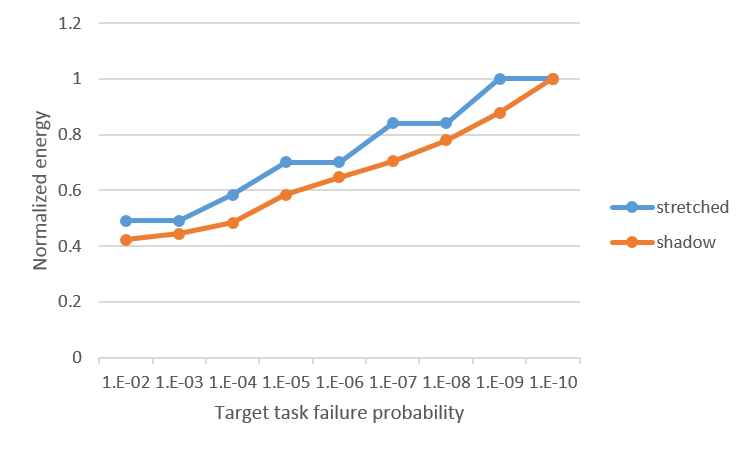
\includegraphics[width=0.45\columnwidth]{Figures/energy_vs_failure_10_100}
		} 
		\subfigure[CPU frequency]
		{
			\label{fig:speed_failure_10_100}
			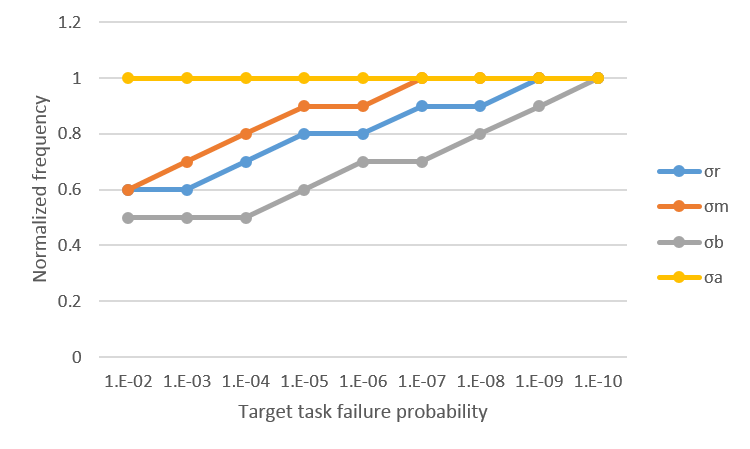
\includegraphics[width=0.45\columnwidth]{Figures/speed_vs_failure_10_100}
		} 
	\end{center}
	%\vskip -0.22in 
	\caption{Impact of target task failure probability on frequency assignment and energy consumption}
	\label{fig:failure_impact}
\end{figure}

\begin{figure}[!t]
	\begin{center}
		\subfigure[Energy consumption]
		{
			\label{fig:en_util_10}
			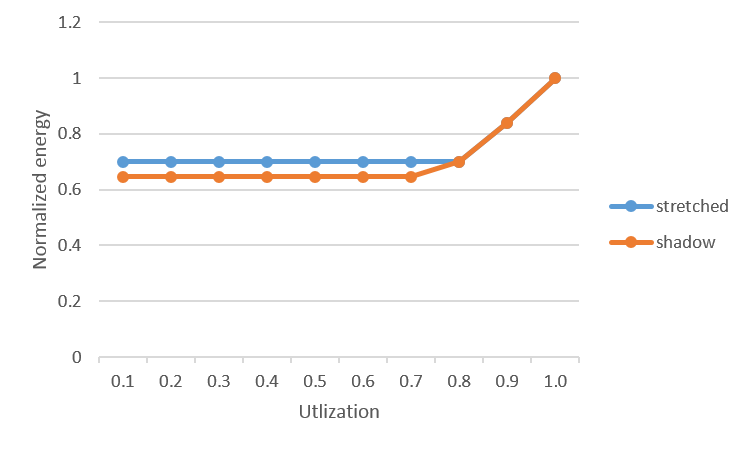
\includegraphics[width=0.45\columnwidth]{Figures/energy_vs_uti_10}
		} 
		\subfigure[CPU frequency]
		{
			\label{fig:speed_util_10}
			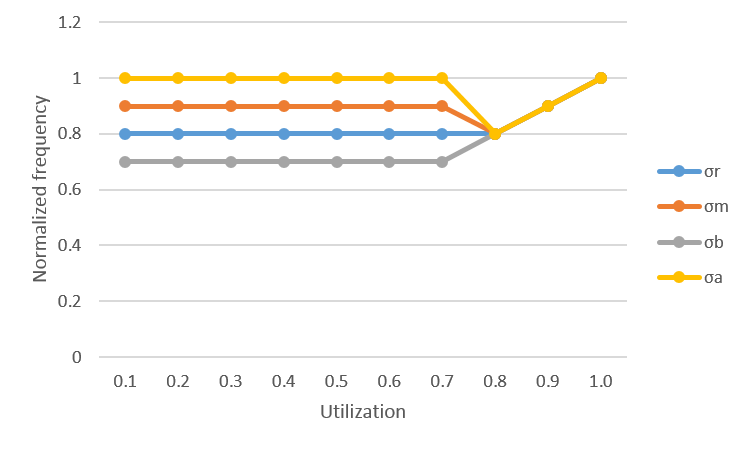
\includegraphics[width=0.45\columnwidth]{Figures/speed_vs_uti_10}
		} 
	\end{center}
	%\vskip -0.22in 
	\caption{Impact of utilization on frequency assignment and energy consumption}
	\label{fig:utilization_impact}
\end{figure}




\section{Simulation}
\label{sec:sim}
In order to verify the analytical models, we develop an event-driven simulator for shadow replication with CSIM. 
The architecture of the simulator is shown in Fig.~\ref{fig:sim}. The simulator has 5 CSIM processes and they interact
with each other through CSIM events. The first CSIM process is Global Coordinator that launches all other CSIM processes
and output statistics after the simulation is done. Failure Injector is another CSIM process that injects failures to 
the running task instances according to a specified failure distribution. Main and Shadow are two processes that "execute" 
the real-time task. They will run at the frequencies derived from analytical models. Finally, we have a Task coordinator
 that terminates the Shadow process if the Main process finishes, or speed up the Shadow process if the Main process 
fails. 
The input to the simulator are the parameters for the task, failure, and frequency. After each simulation, the energy 
consumption is reported. 


\begin{figure}[!t]
	\begin{center}
    	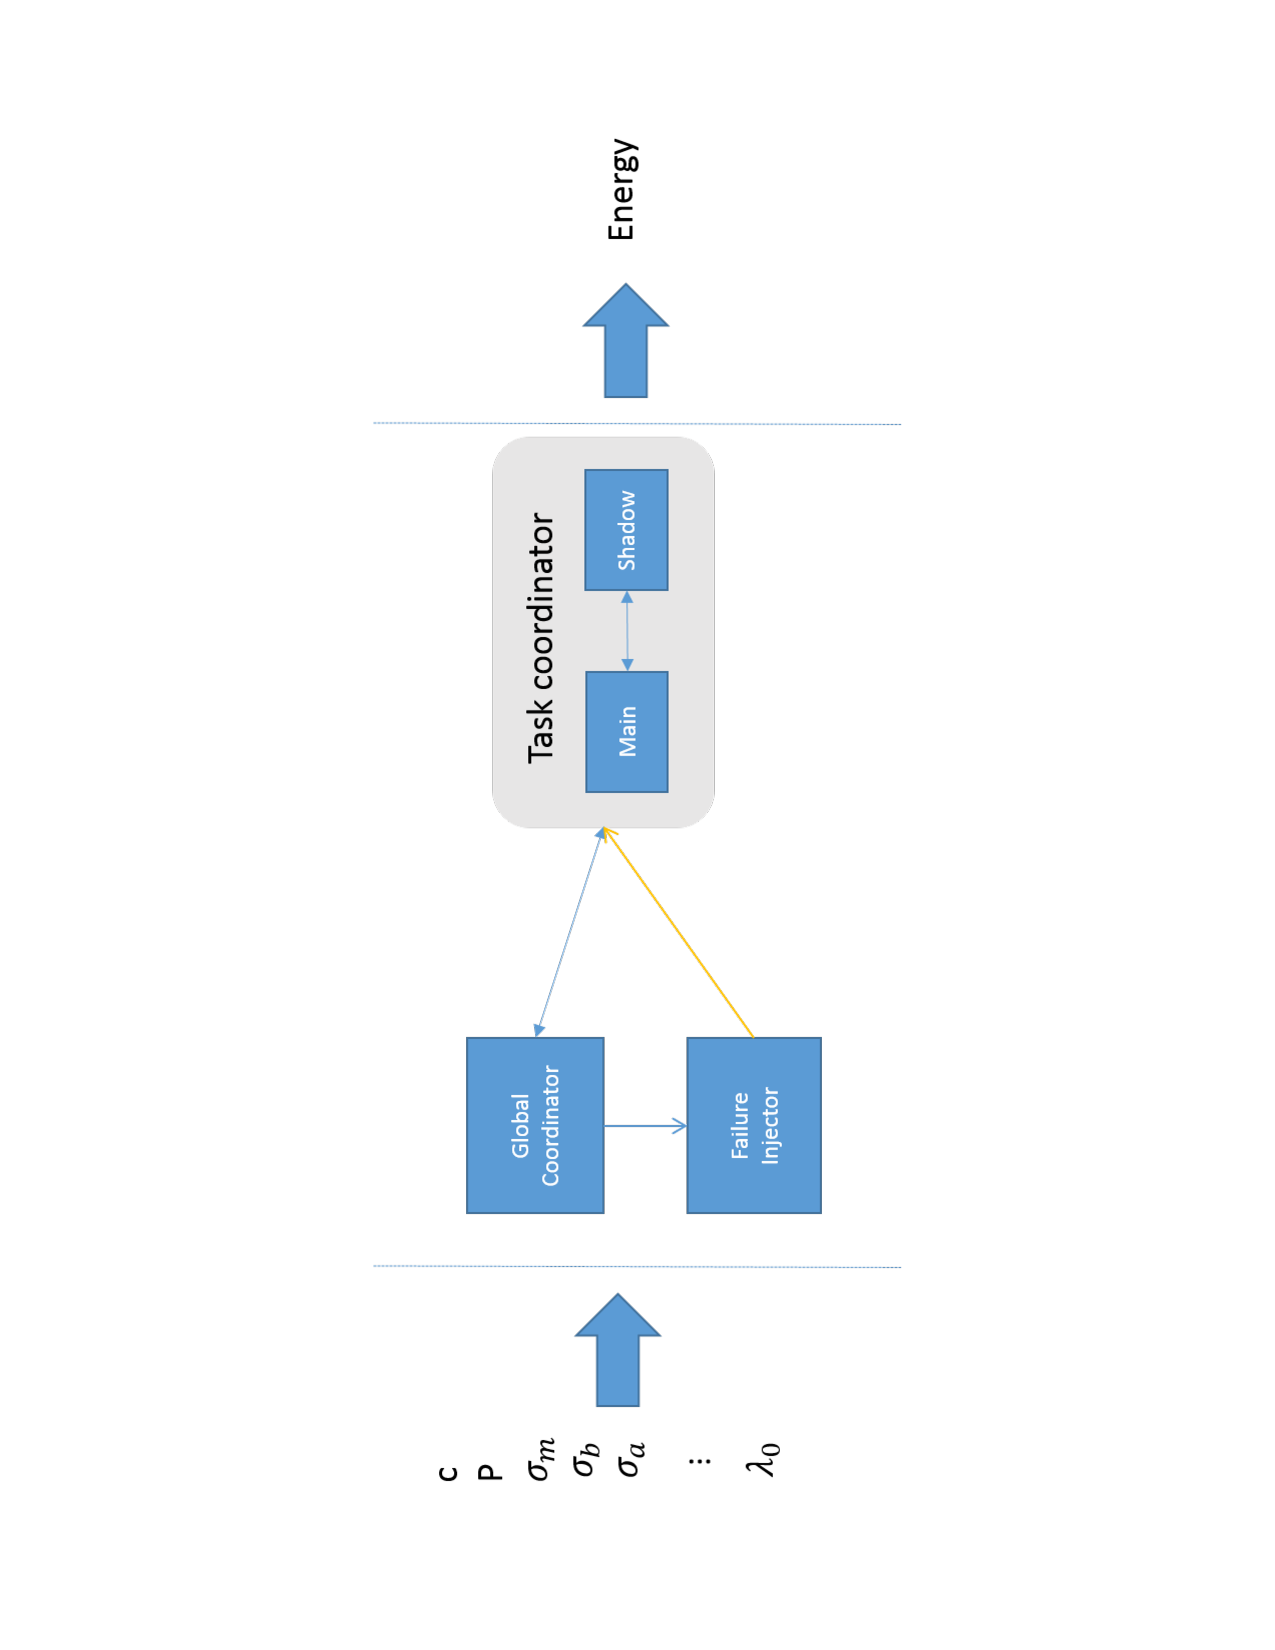
\includegraphics[width=0.5\columnwidth]{Figures/simulator}
	\end{center}
	\caption{Simulator architecture}
	\label{fig:sim}
\end{figure}

Using the simulator, we repeat the study for shadow replication as shown in Fig.~\ref{fig:failure_impact}  and Fig.~\ref{fig:utilization_impact}. 
The results obtained from our simulation are shown in Fig.~\ref{fig:comparison} as the orange lines, and the analytical results are shown as blue dotted lines. 
Each data point is the average of 20 runs. Due to the very low failure rate ($\lambda_0=10^{-6}$), we only see one failure during all the simulation runs. It is clear from Fig.~\ref{fig:comparison} that the results from simulation closely match our previous results from analytical models.

\begin{figure}[!t]
	\begin{center}
		\subfigure[Impact of target task failure probability]
		{
			\label{fig:com_failure}
			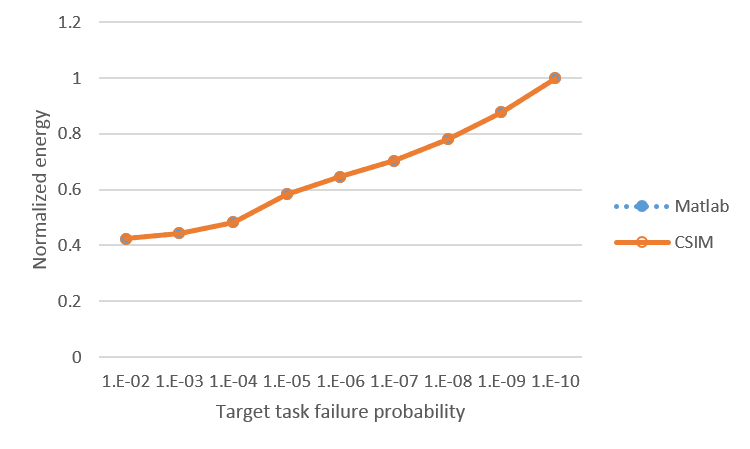
\includegraphics[width=0.45\columnwidth]{Figures/matlab_energy_vs_failure_10_100}
		} 
		\subfigure[Impact of utilization]
		{
			\label{fig:com_uti}
			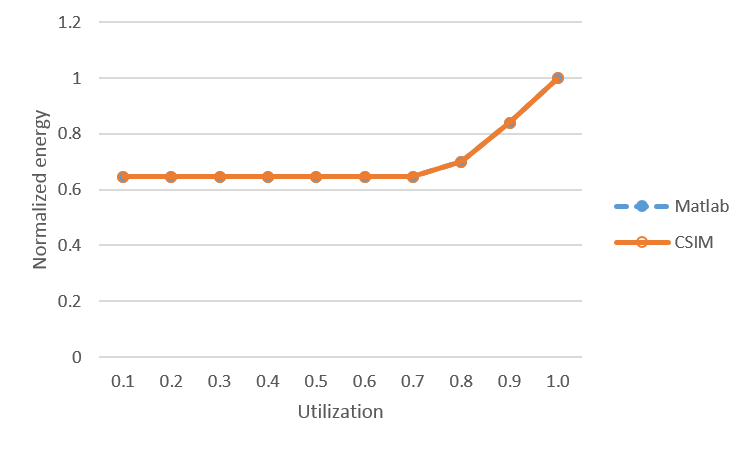
\includegraphics[width=0.45\columnwidth]{Figures/matlab_energy_vs_uti_10}
		} 
	\end{center}
	%\vskip -0.22in 
	\caption{Comparison between analytical and simulation results. $c=10ms$, $f_{min}=0.5$, $\alpha=0.1$, $d=4$, $\lambda_0=10^{-6}$.}
	\label{fig:comparison}
\end{figure}




%\section{Methodology}
%\label{sec:progress}
%\begin{figure*}[!t]
	\begin{center}
		\subfigure[No Failure]
		{
			\label{fig:sc_no_fail}
			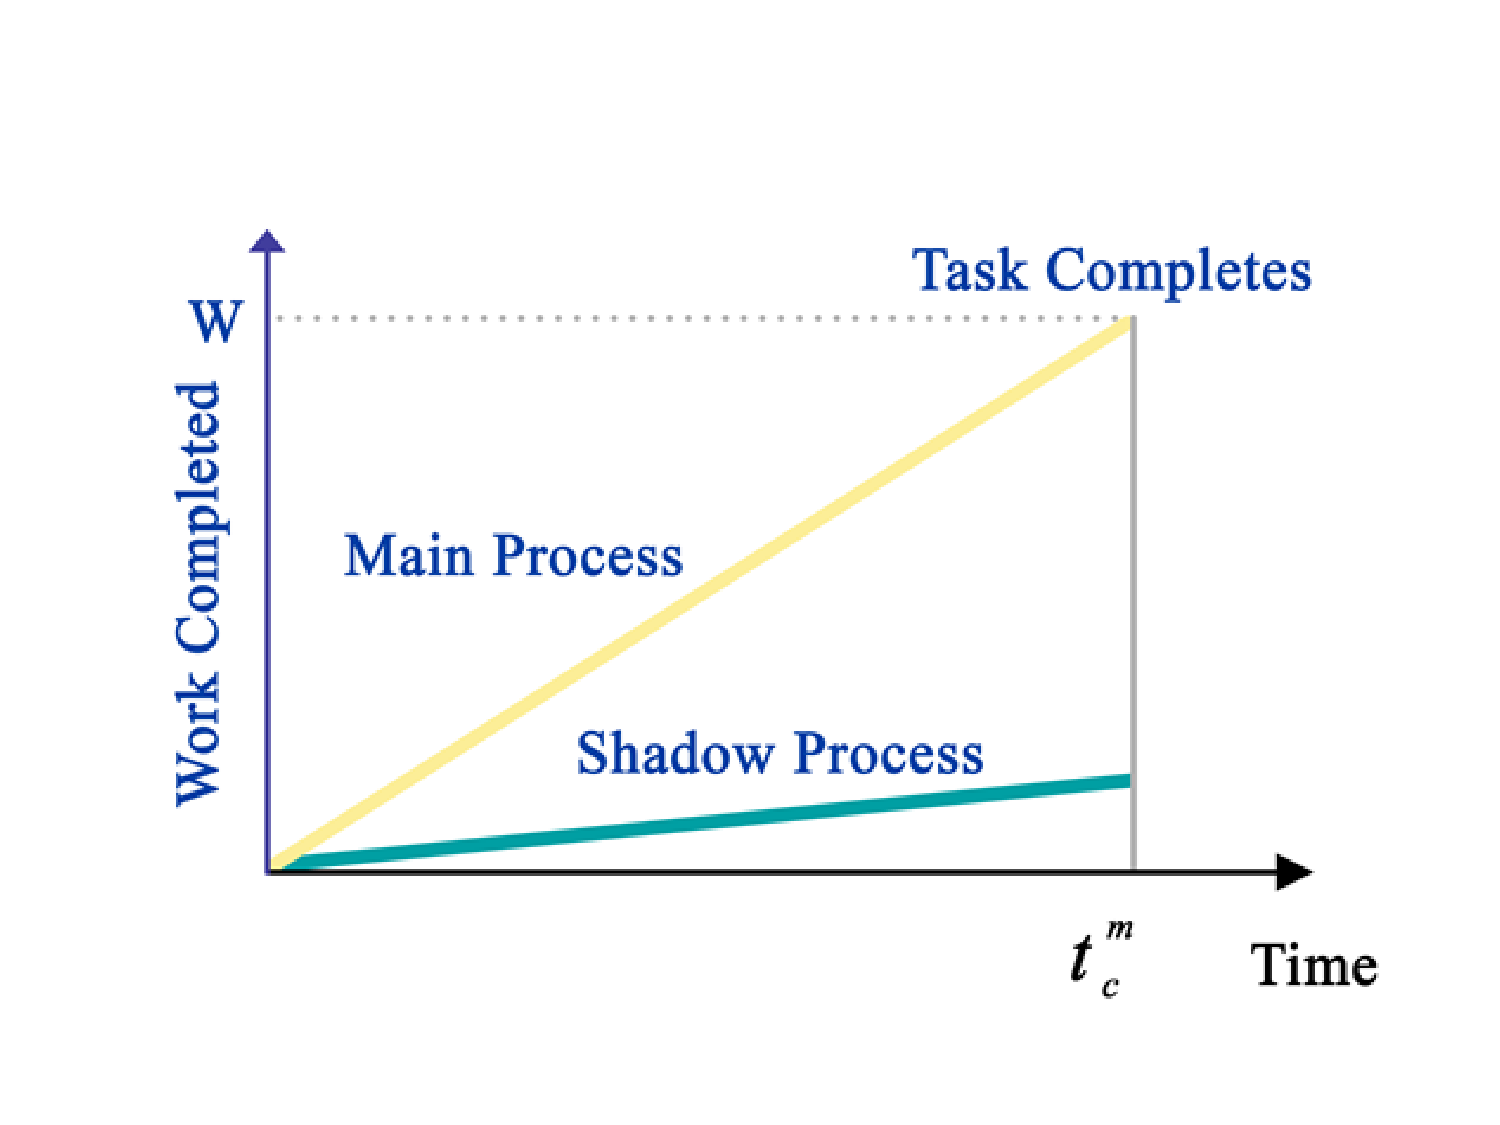
\includegraphics[width=0.32\textwidth]{Figures/example1.pdf}
		}
		\subfigure[Shadow Process Failure]
		{
			\label{fig:sc_shadow_fail}
			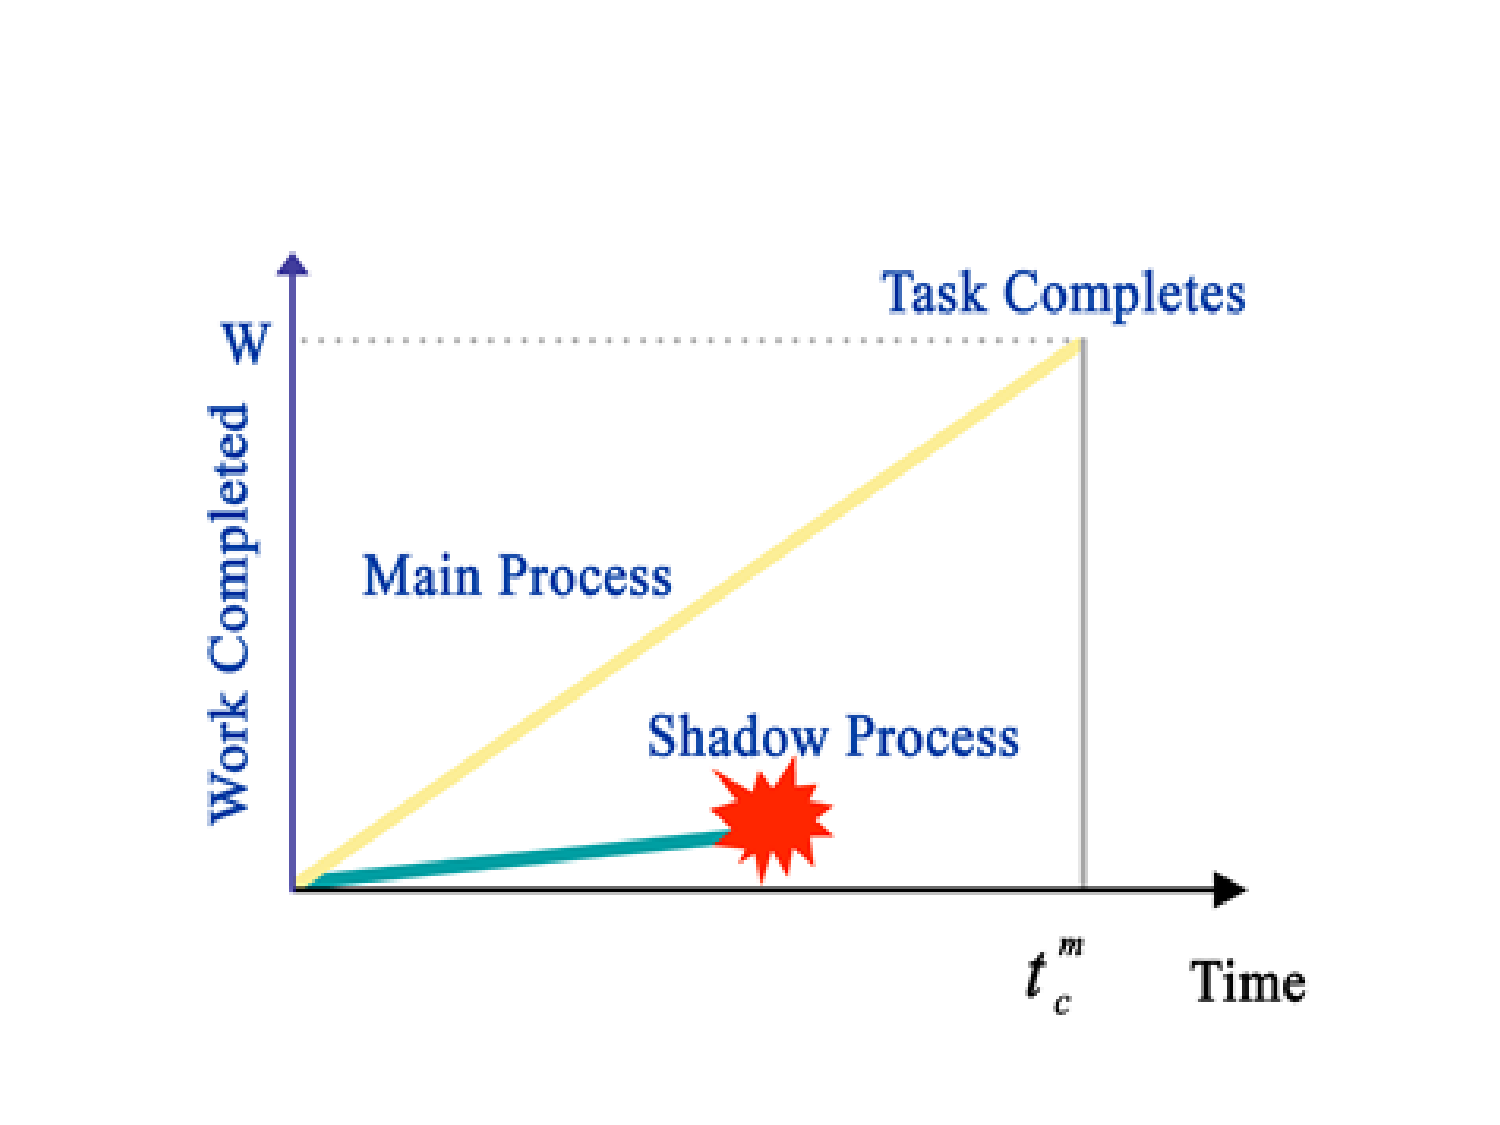
\includegraphics[width=0.29\textwidth]{Figures/example3.pdf}
		}
		\subfigure[Main Process Failure]
		{
			\label{fig:sc_main_fail}
			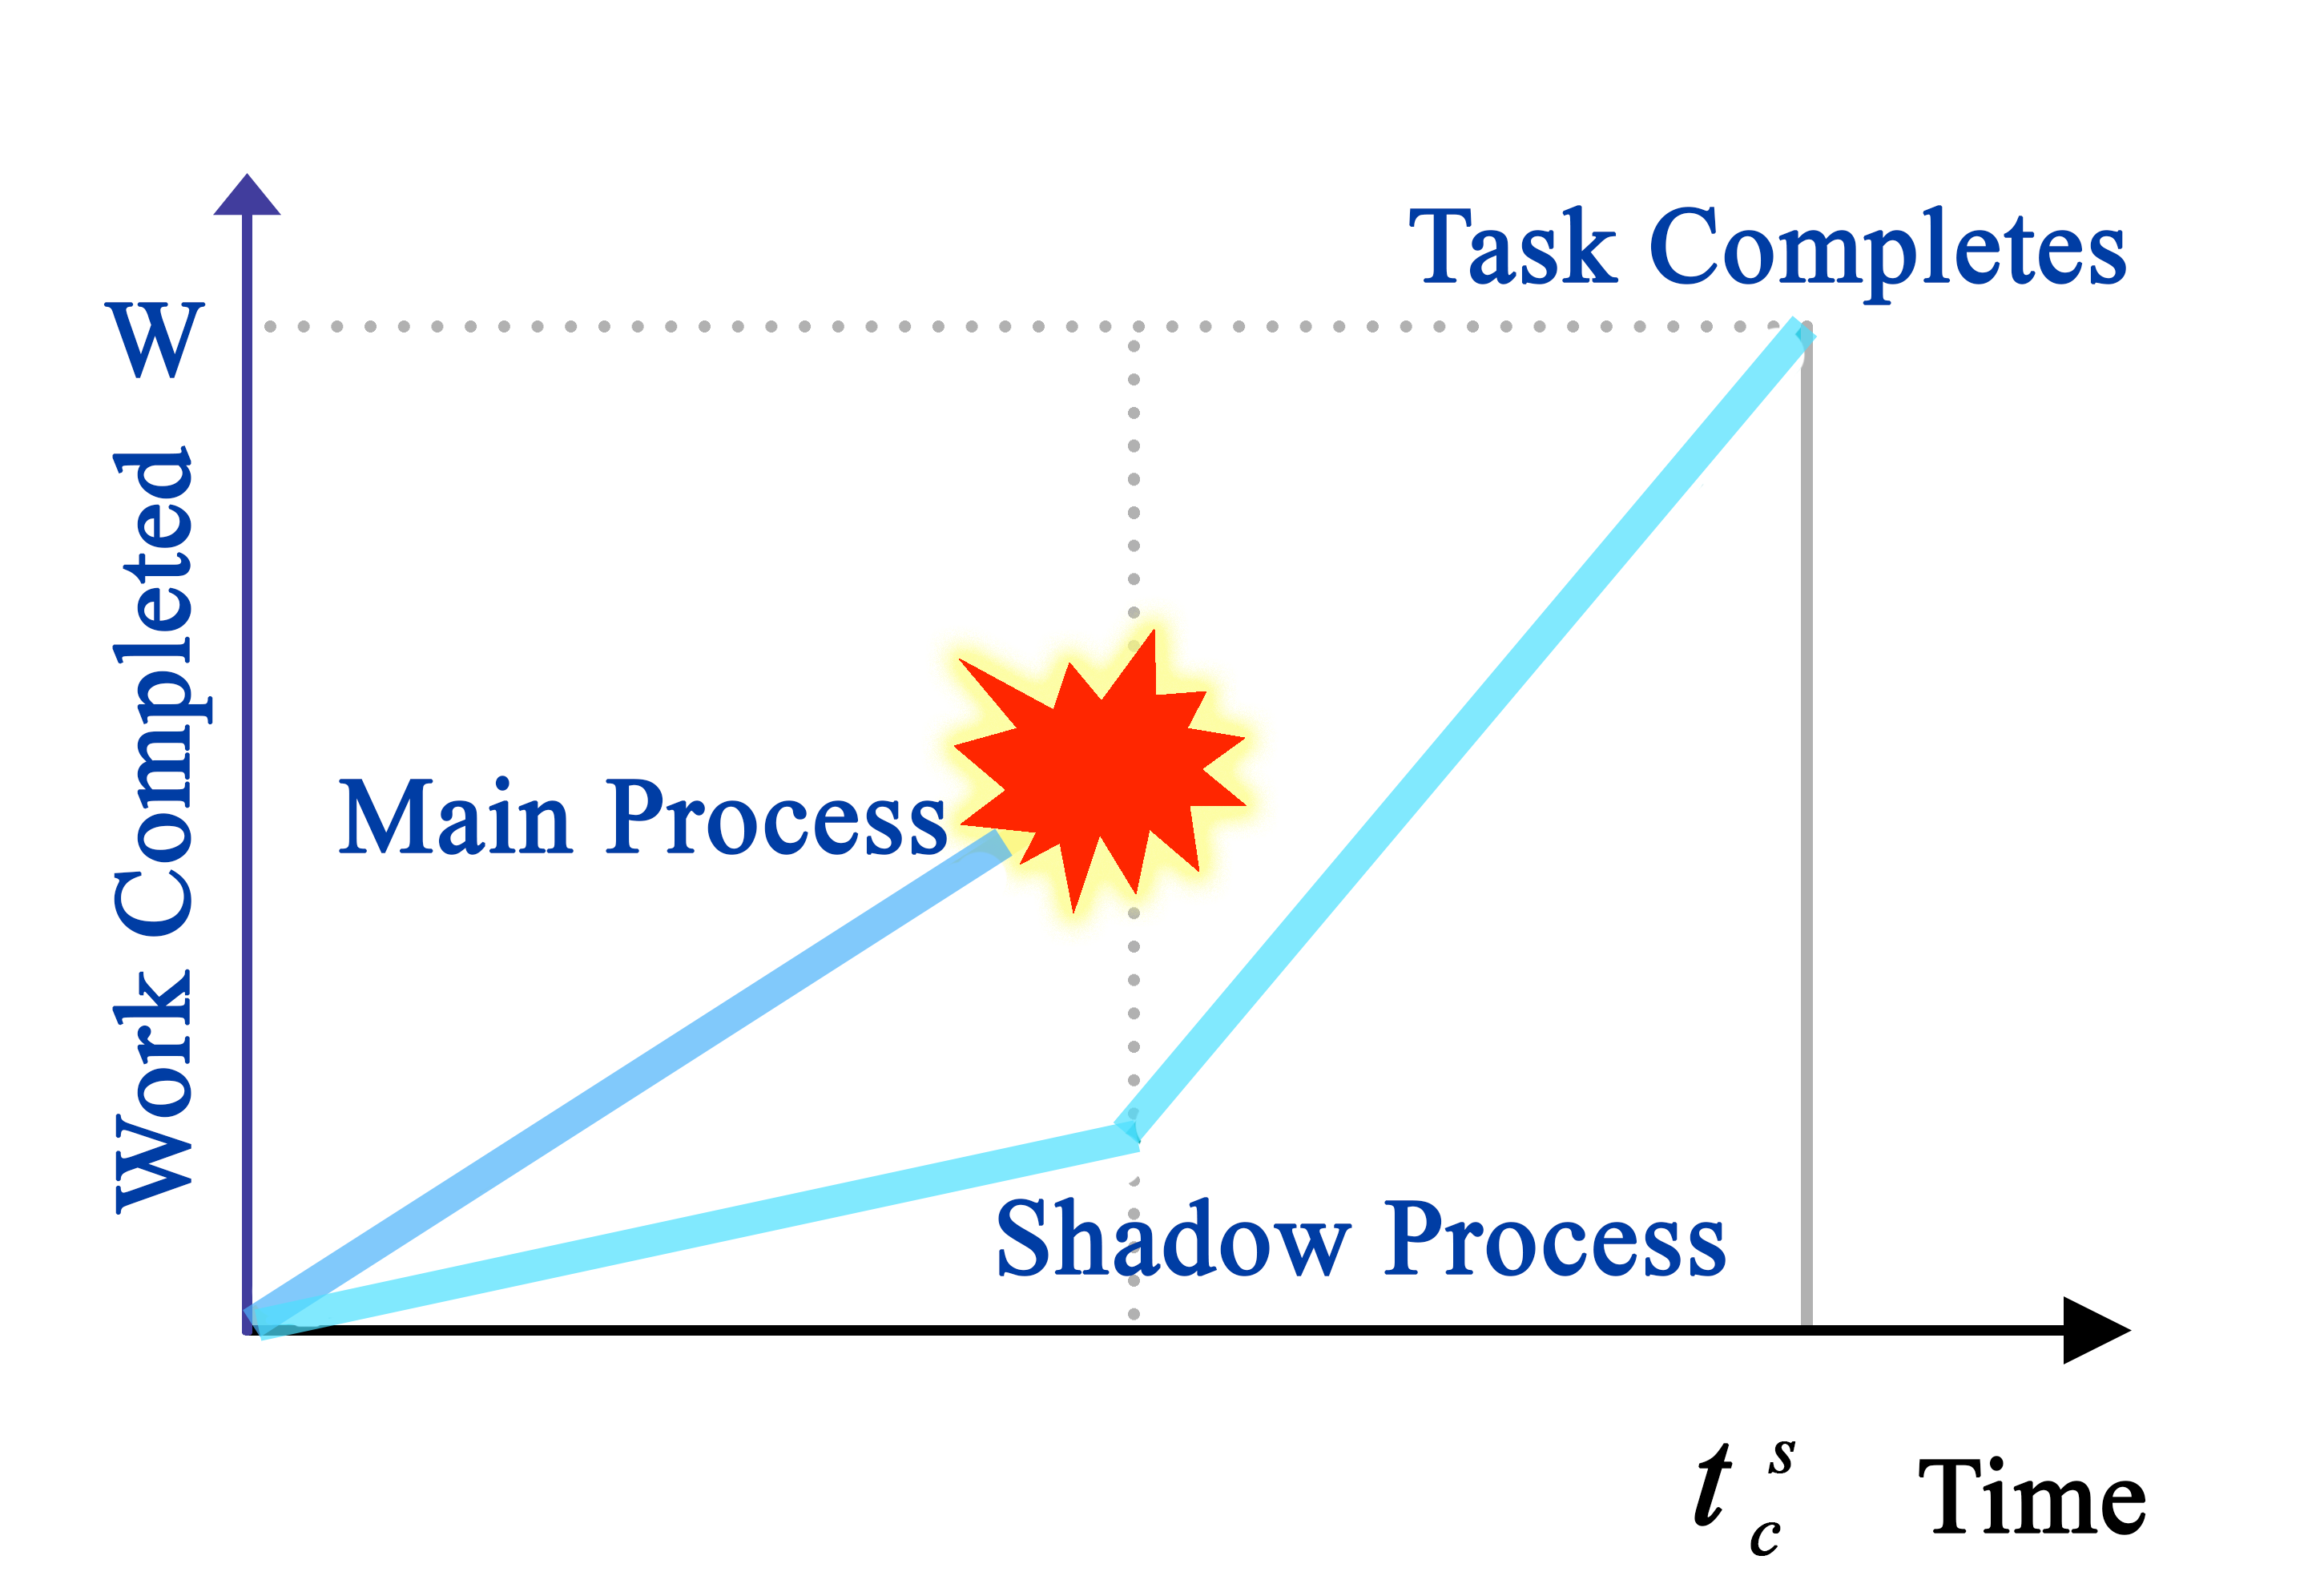
\includegraphics[width=0.33\textwidth]{Figures/example2.png}
		}
	\end{center}
	\caption{Shadow Replication with a single shadow process.}
	\label{fig:sc_overview}
\end{figure*}


So far, we have accomplished the following goals:
\begin{itemize}
	\item A formal definition of the Shadow Replication fault tolerance framework;

	\item Development of a profit-based analytical model to explore the applicability of
	  Shadow Replication to Cloud Computing, and to determine the optimal
	  execution rates of all task instances to maximize profit as well as to reduce energy consumption;

	\item Development of an event-driven simulator to verify the above analytical model;

	\item A comprehensive evaluation using both the analytical model and simulator to analyze the profit and 
	energy savings achievable by Shadow Replication, compared to existing fault tolerance approaches.
\end{itemize}

We have submitted three papers on this work. \cite{cui_en7085151} is published in Energies 7, no. 8 (2014) and \cite{cui_closer_2014} is accepted to CLOSER 2014. Our third paper is currently under review.

\subsection{Shadow Replication}
The basic tenet of Shadow Replication is to associate with each main instance a suite of ``shadows" whose size depends on the criticality of the application and its performance requirements, as defined by the SLA. Each instance is executed with a process. 
To overcome potential failures, each process
executes on a separate computing node.

Formally, we define the Shadow Replication fault tolerance framework as follows:
\begin{itemize}
	\item A main process, $P_m(W$, $\sigma_m)$, that executes at the rate of $\sigma_m$ to complete a task of size $W$;
	\item A suite of shadow processes, $P_s(W$, $\sigma_b^s$ , $\sigma_a^s)$ $(1 \le s \le S)$, where $S$ is the size of the suite. The shadow processes execute on separate nodes, and start execution simultaneously with the main process at rate $\sigma_b^s$. Upon failure of the main process, all shadows switch their rates to $\sigma_a^s$, with one shadow process designated as the new main process. This continues until the completion of the task.
\end{itemize}

There are several ways to slow down the execution rates of the processes. The one that we are studying is Dynamic Voltage and Frequency Scaling (DVFS), as it is the most straightforward solution. When DVFS is enabled, the CPU frequency (which translates to execution rate) scales proportionally to the voltage. Therefore, decreasing voltage not only reduces power and energy consumption, but also effectively slows down the running processes. 

To illustrate the behavior of Shadow Replication, we use only one shadow process and consider the scenarios depicted in Figure \ref{fig:sc_overview}, assuming at most one process failure. Figure \ref{fig:sc_no_fail} represents the case when neither the main nor the shadow fails. The main process, executing
at a higher rate, completes the task at time $t_c^m$. At this time, the shadow process, progressing at a lower rate, stops execution immediately. Figure \ref{fig:sc_shadow_fail} represents the case when the shadow fails. This failure, however, has no impact on the progress of the main process, which can still complete the task at $t_c^m$. Figure \ref{fig:sc_main_fail} depicts the case when the main process fails while the shadow is in progress. After detecting the failure of the main process, the shadow begins executing at a higher rate, completing the task at time $t_c^s$. Given that the failure rate of an individual node is much lower than
the aggregate system failure, it is very likely that the main process
will always complete its execution successfully, thereby achieving fault tolerance at a significantly reduced cost of energy consumed by the shadow. 

A closer look at the model reveals that Shadow
Replication is a generalization of existing fault tolerance
approaches, namely re-execution and process replication. If the
SLA specification allows for flexible completion time, Shadow
Replication would take advantage of the delay laxity to trade time
redundancy for energy savings. It is clear, therefore, that for a
large response time, Shadow Replication converges to re-execution, as
the shadow remains idle during the execution of the main process and
only starts execution upon failure. If the target response time is
stringent, however, Shadow Replication converges to process replication,
as the shadow must execute simultaneously with the main at the same
rate. The flexibility of the Shadow Replication provides the
basis for the design of a fault tolerance strategy that strikes a
balance between task completion time and energy saving, thereby
maximizing profit.

\subsection{Analytical model and simulator}

One challenge of Shadow Replication resides in determining
jointly the execution rates of all processes, both before and
after a failure occurs, with the objective to minimize energy and
maximize profit. To achieve this, we propose a reward-based analytical
model. In the model, we consider the completion time and energy consumption of executing a cloud job, which is composed of multiple parallel tasks, under different system specifics and failure distributions. The profit for cloud service providers is modeled as the difference between the payment from customers, and expenses for running the cloud job. Afterwards, an optimization problem is formulated to derive the optimal execution rates. For more details of the analytical model, please refer to~\cite{cui_en7085151}. 

To verify the correctness of the analytical model, we build an event-driven simulator using CSim that simulates the behaviors of Shadow Replication under different configurations and with different failure distributions, and then report statistics, such as number of failures encountered, time to completion, and energy consumption. 

\subsection{Preliminary results}
With the analytical model and simulator, we identify several important parameters that impact the energy consumption and profit gains of Shadow Replication, and conduct a series of sensitivity studies correspondingly. %The influential parameters can be classified into three categories, i.e., system specifics, SLA specifics, and job specifics. Further, the system specifics includes static power/dynamic power ratio and failure distribution, the job specifics includes workload and number of tasks, and SLA specifics is mainly targeted job completion time 
The results using both the analytical model and simulation show that Shadow Replication can achieve significant energy savings and profit gains compared to traditional process replication and re-execution, without violating the SLA constraints. %Specifically, we conducted 4  sensitivity studies. 

We first study the sensitivity to static power/dynamic power ratio. In this study, we considered modern systems with static power ratio from 40\% to 70\%. Within this range, Shadow Replication can achieve, on average, 19.3\% more profit than traditional replication, and 28.8\% more than re-execution. In terms of energy, the saving is 15\%-30\%.
The second study is to the targeted job completion time. The results show that targeted job completion time influences the execution strategies of Shadow Replication to a large extent, and the reason is that Shadow Replication would strive to maintain the completion time constraint. When time is critical, Shadow Replication uses both a main and a shadow from the very beginning, in the same manner as traditional replication, to guarantee that task can be completed on time; when time is not critical, it mimics re-execution and starts its shadow only after a failure. The profit gains by Shadow Replication can be as much as 52.8\%.
In the next study, we vary the number of tasks from 100 to 10,000,000. On average, Shadow Replication achieves 59.3\% and 18.4\% more profits than process replication and re-execution, respectively.
Our last study is to assess the sensitivity to failure vulnerability, where we find that increasing the failure vulnerability has the same effect as increasing the number of tasks. 


%\begin{itemize}
%	\item Sensitivity to static power/dynamic power ratio. In this study, we considered modern systems with static power ratio from 40\% to 70\%. Within this range, Shadow Replication can achieve, on average, 19.3\% more profit than traditional replication, and 28.8\% more than re-execution. In terms of energy, the saving is 15\%-30\%.
%	\item Sensitivity to targeted job completion time. The results show that targeted job completion time influences the execution strategies of Shadow Replication to a large extent, and the reason is that Shadow Replication would strive to maintain the completion time constraint. When time is critical, Shadow Replication uses both a main and a shadow from the very beginning, in the same manner as traditional replication, to guarantee that task can be completed on time; when time is not critical, it mimics rexecution and starts its shadow only after a failure. The profit gains by Shadow Replication can be as much as 52.8\%.
%	\item Sensitivity to number of tasks. We considered the number of tasks from 100 to 10,000,000. On average, Shadow Replication achieves 59.3\%, and 18.4\% more profits than traditional replication and re-execution, respectively.
%	\item Sensitivity to failure vulnerability. In this study, we found that increasing the failure vulnerability would have the same effect as increasing the number of tasks. 
%\end{itemize}

To summarize, Shadow Replication can achieve 15\%-30\% energy savings and 20\%-30\% more profit on modern systems\cite{cui_closer_2014}. Furthermore, Shadow Replication would converge to process replication, when target response time is stringent, and to re-execution when target response time is relaxed or when failure is unlikely.


%\section{Future directions}
%\label{sec:future}
%Current results reveal that Shadow Replication is promising for significant energy saving within QoS constraints. The direct benefits include profit gains for cloud service providers and reduced $CO_2$ emission, making Cloud Computing more environment-friendly and more sustainable. Inspired by that, I will be fully committed to solve some challenging questions in the next academic year.
%have several research directions to explore in the future.

The first plan is to further improve the efficiency of Shadow Replication for tightly-coupled jobs. My current design works well for loosely-coupled jobs, such as MapReduce jobs, where synchronization among tasks is minimized. 
 In a tightly-coupled job, however, even a very short recovery time may be amplified by the frequent synchronizations,  
 %the parallel tasks need to synchronize with each other frequently. If one task fails, others have to stop and wait for it to catch up. Shadow Replication is able to reduce the catch-up time, because it runs multiple instances of each task, and if one fails, others can speed up to catch up soon. However, the idle time during the catch-up is still a waste, 
 resulting in a delay in the job completion time. In order to minimize this effect and further improve performance, I plan to explore the potential benefits of a new approach, referred to as ``Leaping Shadows". The idea is to take advantage of the recovery time and align the execution states of the slow shadow processes with their faster main processes to achieve forward progress. Remote Direct Memory Access (RDMA) is a possible way to implement Leaping Shadows, but how to efficiently use it needs further research. I plan to finish this work in three months. 

The next research direction is to evaluate the feasibility and performance of using process collocation in Shadow Replication. My current work assumes Dynamic Voltage and Frequency Scaling (DVFS) in controlling the execution rates. The effectiveness of DVFS, however, may be markedly reduced in computational platforms that exhibit saturation of the processor clock frequencies or large static power consumption. An alternative is to collocate multiple processes on a single computing node, while keeping the node running at the maximum rate. Time sharing can then be used to achieve the desired execution rates.
%Process collocation is an alternative approach to slowing down the process execution rate. By collocating multiple processes on the same computing node, the execution rate of each process is proportional to its time share on the node. For Cloud Computing, process collocation may be a better choice than DVFS as the computing nodes in the cloud datacenters are usually time shared by multiple virtual machines. 
%
The two alternatives are equivalent in terms of completion time, since they have the same effect on the execution rate control. In terms of energy, however, each of them has its own advantage. Process collocation requires less hardware resources and this reduces the energy linearly, while DVFS uses more hardwares but can reduce energy superlinearly. It needs further analysis to determine which alternative consumes less overall energy. Furthermore, more efforts are needed to study the potential issues with process collocation, such as correlated failures and collocation overhead. This will take approximately three months to complete. 

The last and most challenging step is to build a prototype, in order to experimentally evaluate the performance of Shadow Replication using real life applications. This effort includes the design and implementation of a distributed software library that supports the main components of Shadow Replication, including process collocation, required consistency protocols, message logging and message forwarding protocols, and execution state transfer in support of Leaping Shadows. For Shadow Replication to be scalable and efficient, it is necessary to minimize its overhead to the normal execution of the running processes as well as to the operating system. This work will take approximately six months to accomplish. 




%There are two potential ways to tune the execution speed of the processes. One is to use Dynamic Voltage and Frequency Scaling (DVFS) to control the execution frequency of the CPU, and the other is to colocate multiple processes on the same node and execute them in a time sharing manner. So far, I have studied the performance of Lazy Shadowing using DVFS. Exploring Lazy Shadowing with time sharing is still under way. 


\section{Conclusion}
\label{sec:conclusion}
%Current fault-tolerance approaches rely exclusively on either time or hardware redundancy for recovery. Rollback recovery  exploits time redundancy but can incur significant delay and high energy cost. On the other hand, process replication relies on hardware redundancy and requires a significant increase in resources and  power consumption.

In this paper, we propose Rejuvenating Shadows as a novel power-aware fault tolerance model, which guarantees forward progress, maintains consistent level of resilience, and minimizes implementation complexity and runtime overhead. Empirical experiments demonstrated that the Rejuvenating Shadows model outperforms in-memory checkpointing/restart in both execution time and resource utilization, especially in failure-prone environments.

Leaping induced by failure has proven to be critical in reducing the divergence between a main and its shadow, 
%with respect to workload execution.
%Consequently, the time to recover from subsequent failures is reduced significantly. 
thus reducing the recovery time for subsequent failures. Consequently, the time to recover from a failure increases with failure intervals.  
Based on this observation, a proactive approach is to ``force" leaping when the divergence between a main and its shadow exceeds a specified threshold. 
In our future work, we will further study this approach to determine what behavior triggers forced leaping in order to optimize the average recovery time. 

%we will study forcing the shadDuring experimentation we noticed the problem that recovery time in Rejuvenating Shadows can become substantial when the failure interval is large (Figure~\ref{fig:single_failure}). To deal with this issue, we are studying the idea of ``forced leaping", which borrows the idea from periodic checkpointing and forces a leaping whenever failure has been absent for a long time, in order to reduce the divergence between mains and shadows. Optimal intervals for forced leaping will be explored to balance between runtime overhead and failure recovery overhead. 

%In the future we plan to explore the integration with fault prediction techniques and the viability of dynamic and partial shadowing for platforms where nodes exhibit different ``health" status, e.g., some nodes may be more reliable while others are more likely to fail~\cite{gainaru2012fault}. 
%With this taken into account, we can apply dynamic scheduling of shadows only for mains that are likely to fail, to further reduce the resource requirement. 
%Another future direction is to study complier-assisted program slicing for fault detection. Specifically, slices that are fraction of their mains can run lazily as shadows and provide fault detection capability with reasonable coverage. 





%\section*{Acknowledgments}


%The author would like to thank Dr. Bryan Mills for his work in developing the initial analytical model (modeling of a single task) for Shadow Computing with DVFS. For clarification, the author performed all the other work presented in this paper.

\bibliography{report}

\bibliographystyle{IEEEtran}



% Following is a new environment, {scilastnote}, that's defined in the
% preamble and that allows authors to add a reference at the end of the
% list that's not signaled in the text; such references are used in
% *Science* for acknowledgments of funding, help, etc.

%\begin{scilastnote}
%\item We've included in the template file \texttt{scifile.tex} a new
%environment, \texttt{\{scilastnote\}}, that generates a numbered final
%citation without a corresponding signal in the text.  This environment
%can be used to generate a final numbered reference containing
%acknowledgments, sources of funding, and the like, per {\it Science\/}
%style.
%\end{scilastnote}




% For your review copy (i.e., the file you initially send in for
% evaluation), you can use the {figure} environment and the
% \includegraphics command to stream your figures into the text, placing
% all figures at the end.  For the final, revised manuscript for
% acceptance and production, however, PostScript or other graphics
% should not be streamed into your compliled file.  Instead, set
% captions as simple paragraphs (with a \noindent tag), setting them
% off from the rest of the text with a \clearpage as shown  below, and
% submit figures as separate files according to the Art Department's
% instructions.


%\clearpage

%\noindent {\bf Fig. 1.} Please do not use figure environments to set
%up your figures in the final (post-peer-review) draft, do not include graphics in your
%source code, and do not cite figures in the text using \LaTeX\
%\verb+\ref+ commands.  Instead, simply refer to the figure numbers in
%the text per {\it Science\/} style, and include the list of captions at
%the end of the document, coded as ordinary paragraphs as shown in the
%\texttt{scifile.tex} template file.  Your actual figure files should
%be submitted separately.



\end{document}




















